%%%%%%%%%%%%%%%%%%%%%%%%%%%%%%%%%%%%%%%%%%%%%%%%%%%%%%%%%%%%%%%%%%%%%%%%%
%
% Purpose: Inspections, Tests, and Metrics for JSC Engineering Orbital Dynamics (JEOD)
%
%
%
%
%%%%%%%%%%%%%%%%%%%%%%%%%%%%%%%%%%%%%%%%%%%%%%%%%%%%%%%%%%%%%%%%%%%%%%%%%

\chapter{Inspections, Tests, and Metrics}\hyperdef{chapter}{ivv}{}\label{ch:ivv}

\section{Inspections}
\inspection{Documentation}\label{inspect:documentation}
This document combined with the \hyperTutorial\ and the JEOD model documentation
set listed in table~\ref{tbl:modeltree} satisfies the requirement~\ref{reqt:documentation}.
Each document has been reviewed by a technical editor and a JEOD team member
other than the author for consistency and clarity.

\inspection{JEOD Coding Standards}\label{inspect:code}
The JEOD source code satisfies the coding standards requirement \ref{reqt:jeod_code}.
This has been confirmed with internal JEOD code reviews, through the use of third
party tools, such as doxygen, and with scripts which flag non-compliant code.

\section{Tests}
\subsection{Integrated  Validation Introduction}
To assure the user and any clients that the JEOD simulation software is valid,
verification and validation through a full empirical comparison of JEOD is required.
Verification of the software involves checking the numerical output of the simulation
against precision orbit ephemeris data from tracked vehicle data (orbit fitting is
the method of generating a precise spacecraft orbit from measured data~\cite{VMcC}).
Integrated Validation of JEOD is a viability demonstration that the software models
met the reasonable requirements of the overall project. It combines with the unit
testing given in the models and should serve as assurance that the software output
can be trusted and a metric for the software's accuracy.

Verification and Validation provide a quantitative measure of the numerical accuracy
of the trajectory generation. Figures of merit from the comparisons for the radial,
in-track and cross-track (the RSW coordinate frame positions are presented in
appendix \ref{ap:rsw}).  For this validation presentation no predetermined pass-failure
criteria can be stated, only the RSW errors stated as metric of measure. The values
of initial measurement orbit fit errors for position are given in the appendix list
of state vectors along with the errors in velocity estimation when given (though all
state vector fit errors are not always available).

The top level JEOD verif directory contains a set of integrated simulations that comprise
the JEOD package validation suite.  These simulations, which can be found in the directory
Integrated\_Validation, consist of the following suite of cases for the public release
version of JEOD:
\begin{itemize}
\item A Lunar orbit simulation to precision orbit ephemeris comparison.
\item A Earth hyperbolic orbit simulation to precision orbit ephemeris comparison.
\item A Mars hyperbolic orbit simulation to precision orbit ephemeris comparison.

\end{itemize}

And with the following additional cases for the NASA internal release version:
\begin{itemize}
\item A low earth orbit (LEO) simulation to precision orbit ephemeris comparison,
\item A high earth orbit (HEO) simulation to precision orbit ephemeris comparison,
\item A geosynchronous orbit (GEO) simulation to precision orbit ephemeris comparison.
\item A dual vehicle Earth orbit simulation simulation to precision orbit ephemeris comparison.

\end{itemize}

These Integrated Validation simulations produce ASCII recordings in inertial coordinates
which match the measured states (see the Benchmarks \ref{ap:bench}).   The measured
and simulated states are post processed into RSW coordinates to get the radial, in-track
and cross-track errors. Microsoft Excel was used to produce the plots and format the data.

The commonly accepted definition for LEO is for orbits between 160 - 2,000 km above
the Earth's surface. HEO (sometimes called Medium Earth Orbit, MEO) are satellites at
altitudes at or above 2,000 kilometers and below geostationary orbit altitude of 35,786
kilometers.  GEO satellites, at 35,786 kilometers could be labeled as ``high" but are
given the particular name of geostationary or GEO.

In the integrated simulations, orbit propagation has been performed to gain a quantitative
measure of the validity of the JEOD propagation and force models.  Gravitational forces
of a non-spherical Earth, the Moon, Mars, n-body perturbations, solid body tide forces,
radiation pressure, and aerodynamic drag are tested.  Also tested is the underlying
environment modeling in support of the propagation, such as rotation-precession-nutation-polar-motion,
the ephemerides and the MET thermosphere models.  Six sets of measured precision orbits
were obtained to use as measures. Four of the measurement sets are time histories from
CHAMP, ENVISAT, LAGEOS and CLEMENTINE data, and two are initial and final orbit fits for
the ISS and TDRS.  Because of unknown attitude profiles in the following, only the basic
aerodynamics was modeled by way of a coefficient of drag or a ballistic coefficient.  It
should be kept in mind that for low earth orbit satellites, the atmospheric density can
only be modeled to within about 15 percent accuracy due to uncertainties in modeling upper
atmospheric winds when not using free molecular flow (Vallado~\cite{VMcC}).  In this release
of JEOD the GRACE Gravity Model 02 (GGM02C) gravitational field is used as the geopotential
model~\cite{2005JGeod} and~\cite{grace}. The solar activity was obtained from Goddard Space
Flight Center's MSIS web site, see appendix{ap:atmos}.


Note 1: For JEOD, the \docsref{GRAVITY}\ uses a normalization method for a high order and
degree non-spherical gravitational field of the Earth and the Moon.

Note 2: For position errors see Appendix \ref{ap:tdata}, and note that the errors in velocity
state are not always available.

\clearpage

\subsection{LEO:}
\test{Integrated Testing CHAMP}\label{test:champ}
\begin{description}
\item[Introduction:] \ \newline
The Challenging Minisatellite Payload (CHAMP) satellite was launched with a Russian
Cosmos launch vehicle on July 15, 2000 into an almost circular, near polar orbit with
an initial altitude of 454 km. The design lifetime of the satellite system  was 5 years.
CHAMP is a small German satellite with a mission for geoscientific and atmospheric
research and applications, managed by the GeoForschungsZentrumPotsdam (GFZ).
\item[Test Satellite CHAMP:] \ \newline
In 2003 CHAMP was at 400 km during a period of enhanced solar activity, thus this satellite
was a very good choice as a benchmark to measure JEOD modeling of the geopotential and
atmosphere. The measurements were taken in April 2003.
\item[Procedure:]\ \newline
A set of precision fit J2000 state vectors was obtained from GFZ by Blair Thompson~\cite{bt}.
The CHAMP ephemeris files are for three consecutive days in 2003.  Each file contains 30
hours of ephemeris (ECI J2000) in 10 second intervals.  The initial state and orbit environment
at that date are given in appendix table \ref{tbl:champic}.  The GPS fitted orbit data has an
absolute error in position of 5 centimeters or less according to the following journal paper~\cite{Bae}.
The physical characteristics of the vehicle and the aerodynamics ballistic coefficient were
obtained from the GFZ~\cite{G} in Germany -
see: the CHAMP state in \ref{tbl:champic}. For aerodynamics only a simple projected area model was used.
\item[Results:]\ \newline
The results of this test are shown in Figure \ref{fig:1}. The RSW or radial, in-track and
cross-track errors ( see Appendix \ref{ap:rsw}), for a one day propagation are shown in Figure \ref{fig:1}.
The biggest errors are less than 2 meters radial, less than 2 meters cross-track. There is a
secular growth in in-track to less than 6 meters when using GGM02C.  Most of the in-track error
comes from atmospheric modeling.  It is noted here that the GGM02C is used with the full fitted
model order = 200 and degree = 200.  The option to use GGM02C to this maximum order and degree
also tested the gravitational algorithm  model that handles a high order expansion.  The RSW
errors are very acceptable, considering the uncertainties in atmosphere and that GGM02C was
fitted with the IERS RNP model \cite{IERS2003}.  This test takes almost 20,000 sec of CPU time,
and checks may be run at lower order and degree.  This test partially satisfies
\ref{reqt:main_function}, \ref{reqt:rel_states}, and \ref{reqt:sim_interface}.
\newpage
\begin{figure}
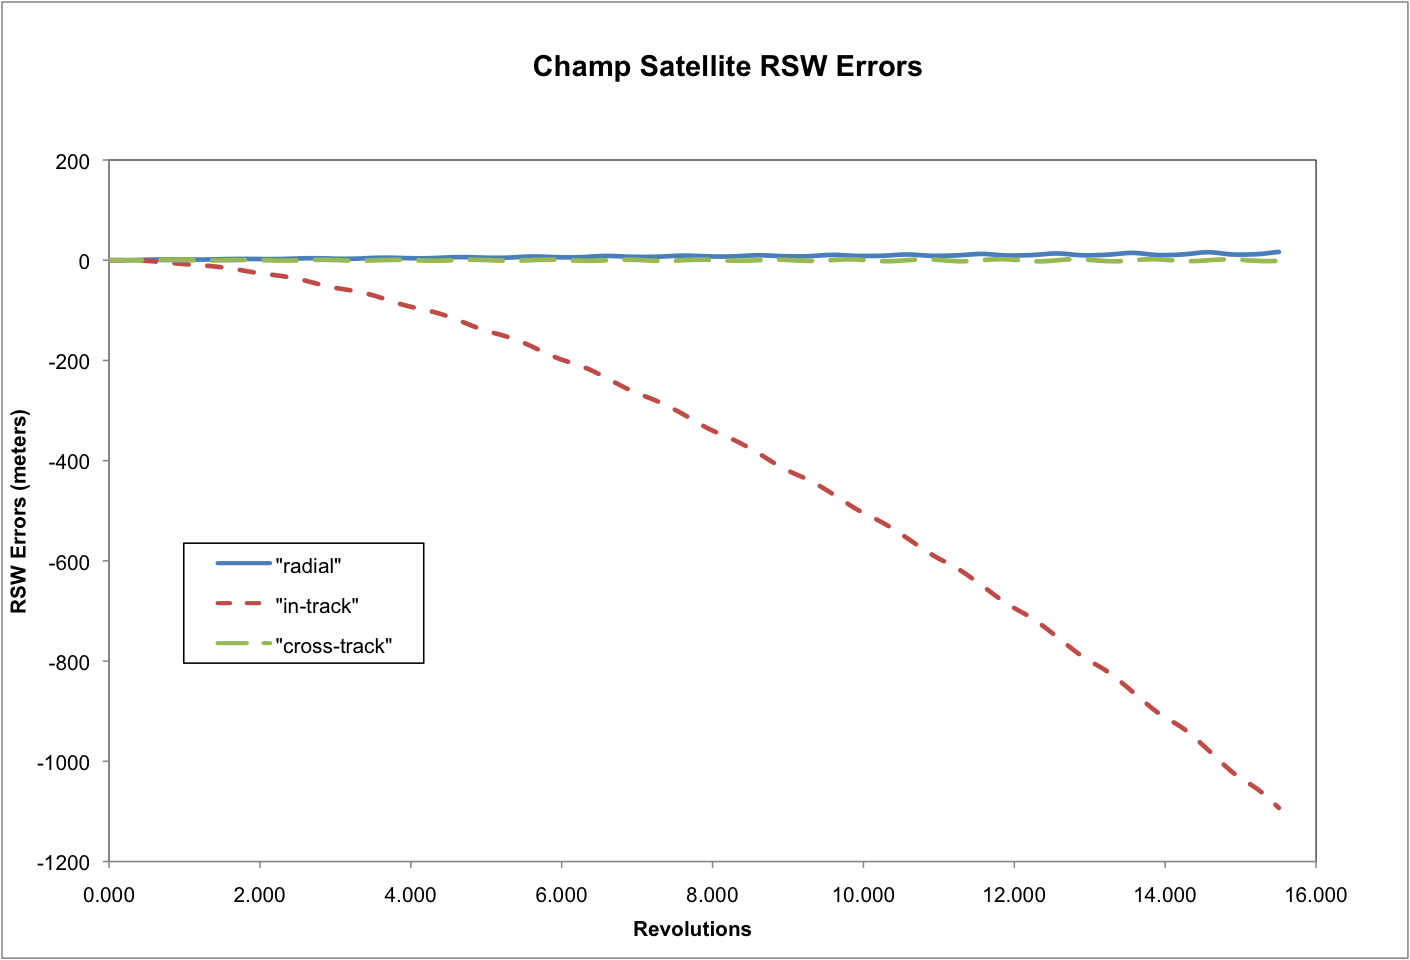
\includegraphics [width=7in]{figs/champ/champ_err.png}
\caption{RSW errors accumulated over a day for the orbit of CHAMP .}
\label{fig:1}
\end{figure}

\end{description}
\clearpage
\newpage

\test{Integrated Testing ISS}\label{test:iss}
\begin{description}
\item[Introduction:] \ \newline
The following test uses the International Space Station (ISS) as test object.  The ISS
is a large articulated spacecraft and hence is subject to large drag perturbations. This
test uses a fixed aerodynamic configuration in the form of a projected area model.  The
purpose is to measure the error produced by JEOD in propagating a large orbiting object
subject to drag.
\item[Requirements:] \ \newline
Quantify the accuracy of JEOD with a large drag spacecraft in low Earth orbit under the
influence of a dynamic atmosphere and non-spherical geopotential as the main perturbing
forces. The aerodynamic configuration for the ISS is fixed throughout the run.
\item[Procedure:]\ \newline
Two precision fit ISS state vectors were obtained from the Mission Operations Directorate,\cite{topo}.
The aerodynamic properties are contained in a document issued by the JSC Engineering
Directorate, Lumpkin~\cite{iss}.  The ISS is in configuration 2A in Torque Equilibrium Attitude.
The initial conditions and physical conditions are shown in appendix table~\ref{tbl:issic}.
The solar activity was obtained at the initial ISS state vector epoch but not changed, even
though the simulation duration is 1 day (this is the interval at which ISS precision states are
obtained~\cite{topo}). Note: Only initial and final orbit fits are available.
\item[Results:]\ \newline
The initial state vector was provided in J2000 inertial coordinates and propagated for one day.
Table \ref{tbl:isserror1} shows the differences in radial, in-track and cross RSW track positions.
The errors in the initial orbit fit are one km in the J2000 intertial Cartesian position coordinates.
The uncertainty in the ISS aerodynamics and the atmosphere density makes a considerable contribution
to the propagated state in the in-track position period for a JEOD simulation.  Though the solar
activity did change during this period it was not large (it would be possible to change a simulation's
solar activity in the input file).  There is also a small contribution due to the geopotential due to
very small unknown errors in using a different Earth Orientation Model than that used to fit GGM02C.
The results are for a geopotential model GGM02C of degree and order 70x70 (there is only a small improvement
in using the 200x200 GGM02C model).  An in-track error of nearly 6 km is the accuracy of using this large
vehicle with an only approximated projected area over the trajectory time line.  This test partially
satisfies \ref{reqt:main_function}, \ref{reqt:rel_states}, and \ref{reqt:sim_interface}.

\begin{table}[htb]
\begin{center}
\caption{ISS RSW Errors for a One Day Orbit Propagation} \vspace{5mm}
\label{tbl:isserror1}
\begin{tabular}{||l|l|l|} \hline
{\bf Component  } & {\bf magnitude of value} & {\bf units } \\ \hline \hline
Radial      & -67.89740334          & meters \\ \hline
In-track    & 6003.885756       & meters  \\ \hline
Cross-track & 33.27854206        & meters \\ \hline
\end{tabular}
\end{center}
\end{table}

\clearpage
\newpage
\end{description}

\subsection{HEO:}
\test{Integrated Testing ENVISAT}\label{test:evi}
\begin{description}
\item[Purpose:] \ \newline
The ENVISAT (Environmental Satellite) satellite is an Earth-observing satellite built
by the European Space Agency. It is in high earth orbit (HEO) with a perigee of 785 km,
an apogee of 791 km and has orbital inclination of 98.6.  ENVISAT carries an array of
nine Earth-observation instruments that gather information about the earth.  The main
home for data collection is the Department of Earth Observation and Space Systems (DEOS)
at Technical University Delft, Delft The Netherlands.
\item[Requirements:] \ \newline
This is classified as HEO because it is an orbit where the atmosphere does not dominate
the translational forces. ENVISAT, near the top edge of the exosphere, the forces due to
the aerodynamic drag are only noticeable during periods of high solar activity otherwise
gravitational and radiation forces are dominant.  It also gives a case where third body
gravitational perturbations are in play.
\item[Procedure:]\ \newline
The initial conditions are given in the appendix for this ENVISAT test \ref{tbl:eviic}.
The data was extracted from the DEOS state vector webserver.  The data is generated
by European Space Operations Centre (ESOC) in Darmstad. The accuracy of the orbit fit
has a root mean sum square of 10 centimeters, and reference for the state error can be
found on ESOC website. The physical characteristics were given by the DEOS webserver
and the aerodynamics from a paper by Doornbos~\cite{ers2}.  J2000 state vectors were
extracted every 10 seconds for 1 day. The full GGM02C gravitational model of order and
degree 200x200 was used in this test.
\item[Results:]\ \newline
The comparison differences between the measured and numerically propagated state vectors
over 24 hours are shown in Figure \ref{fig:3}.  The radial and cross-track differences are
approximately 5 meters after 12 hours, the in-track error drifts noticeable growing to
nearly 10 meters in the same period. The oscillations in all the position errors are mostly
due to perturbations due to the sun and moon. The epoch of the test was during a period of
low solar activity thus the atmosphere has less effect.  It has been shown that under those
conditions, ENVISAT is subject to about 50 percent more force due to radiation forces than
aerodynamic drag forces, Doornbos~\cite{ers2} and Scharroo~\cite{ers1} and~\cite{sch}.
This test partially satisfies \ref{reqt:main_function}, \ref{reqt:rel_states}, and \ref{reqt:sim_interface}.

\begin{figure}
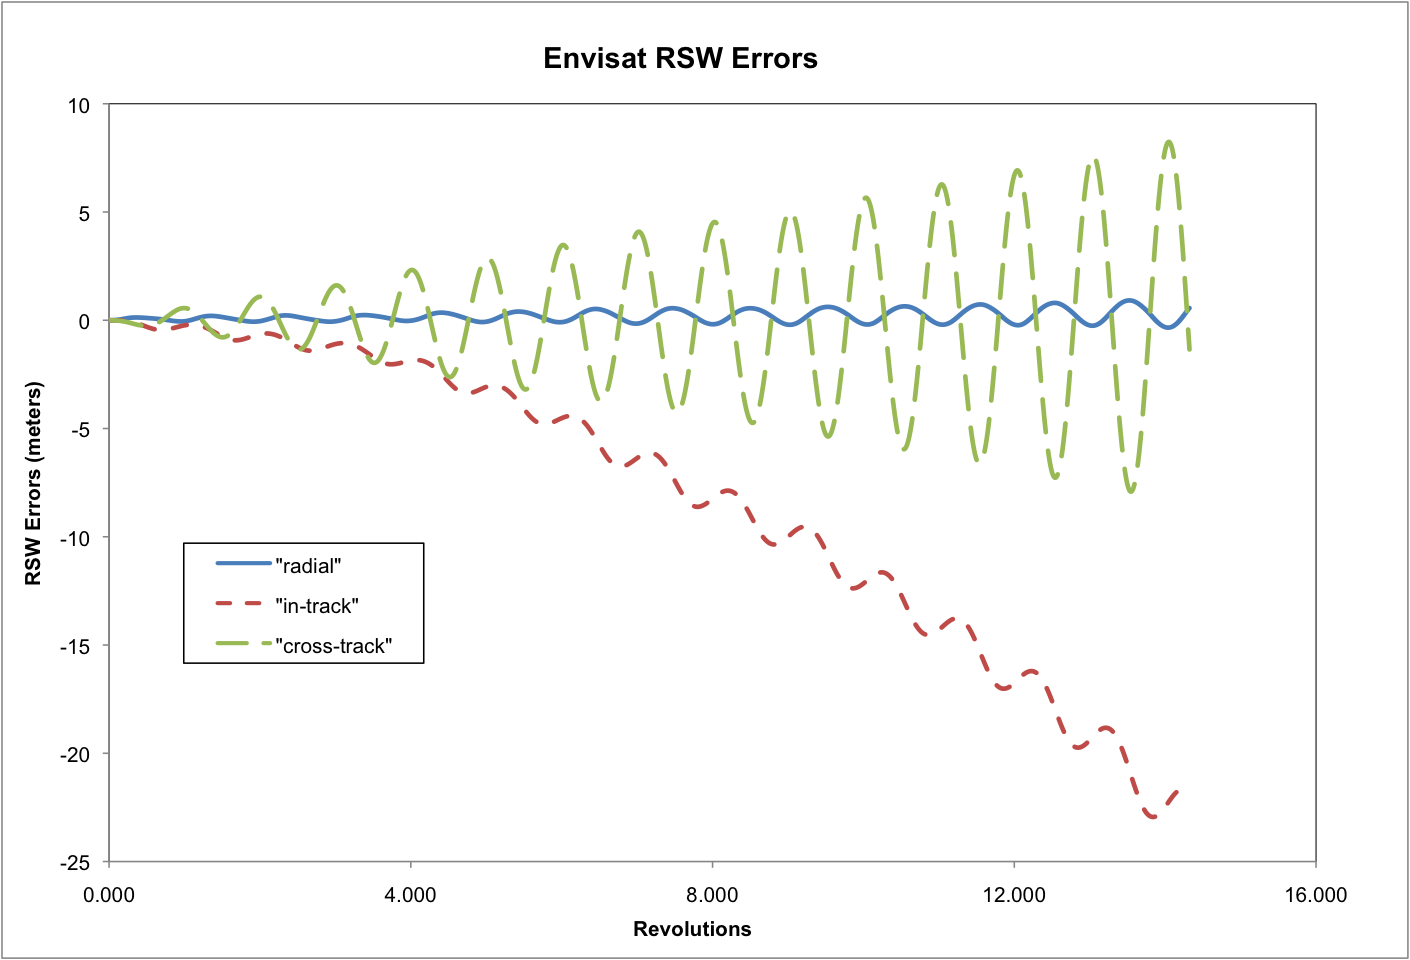
\includegraphics [width=7in]{figs/envisat/envsat_err.png}
\caption{ENVISAT RSW errors between measured and simulated orbit using GGM02C.}
\label{fig:3}
\end{figure}

\clearpage
\pagebreak

\end{description}
\newpage

\test{Integrated Testing Lageos}\label{test:lageo}
\begin{description}
\item[Purpose:] \ \newline
The Lageos satellites are passive vehicles covered with retroreflectors designed to reflect
laser beams transmitted from ground stations. By measuring the time between transmission of
the beam and reception of the reflected signal from the satellite, stations can precisely
measure the distance between themselves and the satellite. These distances can be used to
calculate station positions to within 1-3 cm.
\item[Requirements:] \ \newline
This is a definitive test of a HEO, being at an altitude of 6000 km, because on the Lageos
the forces due to the aerodynamic drag are dominated by radiation pressure. This also gives
a case where third body gravitational perturbations are significant.
\item[Procedure:]\ \newline
The initial conditions are given in the appendix for this Lageos test \ref{tbl:lagic}. The
full GGM02C gravitational model of order and degree 200x200 was used in this test. The data
was provided by Goddard Space Flight Center (private communication Erricos C. Pavlis ~\cite{pav}).
The measurement data by laser tracking is accurate to less than one tenth of a meter, per
NASA TM 104549 ~\cite{lga}.
\item[Results:]\ \newline
The comparison differences between the measured and numerically propagated state vectors over
24 hours are shown in Figure \ref{fig:4}. After 6 revolutions there was a .5 meter error and
1.7 meter cross-track differences. The in-track error of 10.6 meters is attributable to the
Lageos ultra precision orbit fit and some radiation pressure modeling. In addition, there are
error contributions due to the RK4 numerical integrator and other possible non-gravitational
effects such as the albedo of the Earth. Earth shadowing was modeled by a simple cylinder.
Studies have shown that Lageos undergoes many complex non-gravitational forces which JEOD does
not model~\cite{rub}.  This test partially satisfies \ref{reqt:main_function}, \ref{reqt:rel_states},
and \ref{reqt:sim_interface}.
\begin{figure}
\begin{center}
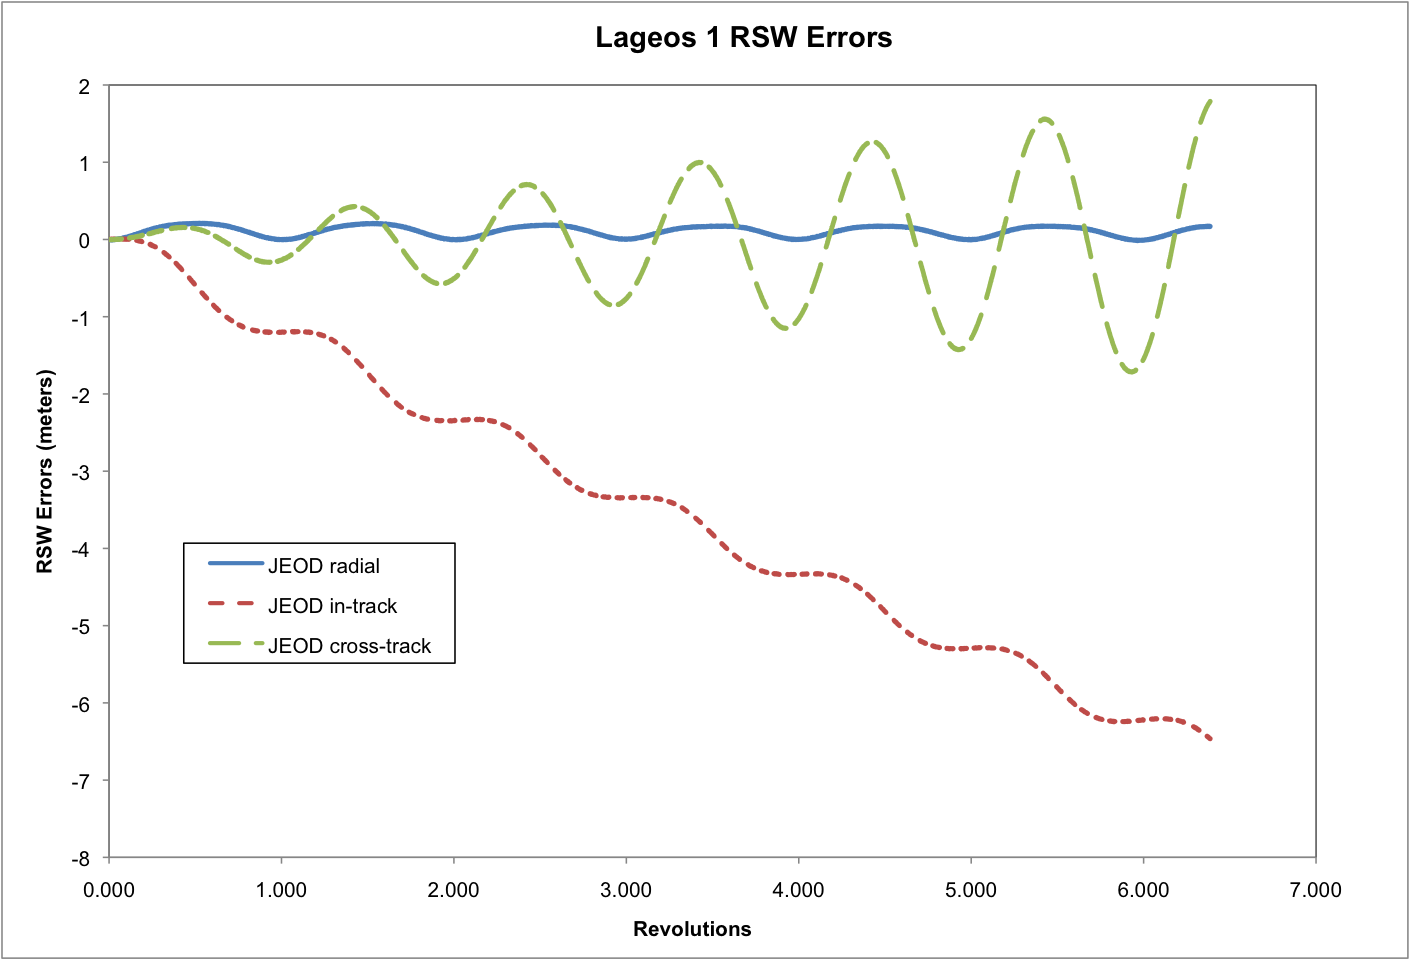
\includegraphics [width=7.0in]{figs/lageos/lageos_err.png}
\end{center}
\caption{Lageos RSW errors between measured and simulated orbit using GGM02C.}
\label{fig:4}
\end{figure}

\clearpage
\pagebreak

\end{description}

\newpage
\subsection{GEO:}
\test{Integrated Testing TDRS}\label{test:tdrs}
\begin{description}
\item[Introduction:] \ \newline
At geosynchronous orbital altitudes the atmospheric drag forces are non-existent,
and the main perturbation forces are the low order geopotential terms, third body
gravitational forces (mainly due to the Moon and Sun) and radiation forces. The
Tracking and Data Relay Satellite (TDRS) is one of a network of communications
satellites used by NASA and other United States government agencies for communication
to satellites or the International Space Station. (For this satellite one finds also,
the name Tracking and Data Relay Satellite System (TDRSS)).
\item[Requirements:] \ \newline
This test is a characterization of the accuracy of a geosynchronous orbit propagation
by comparison to a precision orbit fit. This test mainly measures the influence of
third body perturbations which are dependent on the generation of the JPL ephemerides
and radiation pressure forces.
\item[Procedure:]\ \newline
A precision fit state vector was obtained from JSC's Mission Operations Directorate, \cite{topo}
see the appendix table \ref{tbl:tdrsic}.  These vectors are separated in time by a day.
The accuracy of the TDRS initial state vectors is approximately 1 km in position~\cite{tdrs}.
\item[Results:]\ \newline
The results are shown as plots in Figure \ref{fig:5}. The in-track error reflects a long
propagation of the orbital state by numerical integration. The step size for the Runge Kutta
(order 4) method has a quadratic accumulation of error. GGM02C was used setting order and
degree to 8x8. It is known that radiation pressure makes a contribution to perturbations at
geosynchronous distances, and these are modeled in JEOD. In this case TDRS is a complex object,
thus radiation pressure modeling can only be approximated. The in-track error generated by JEOD
is about 250 m for a one day propagation, and this may be due to radiation pressure. For long
propagations, JEOD will be sensitive to initial position errors of a given state which are of
the order of 1km for this TDRS case. This test partially satisfies \ref{reqt:main_function},
\ref{reqt:rel_states}, and \ref{reqt:sim_interface}.

\begin{figure}
\begin{center}
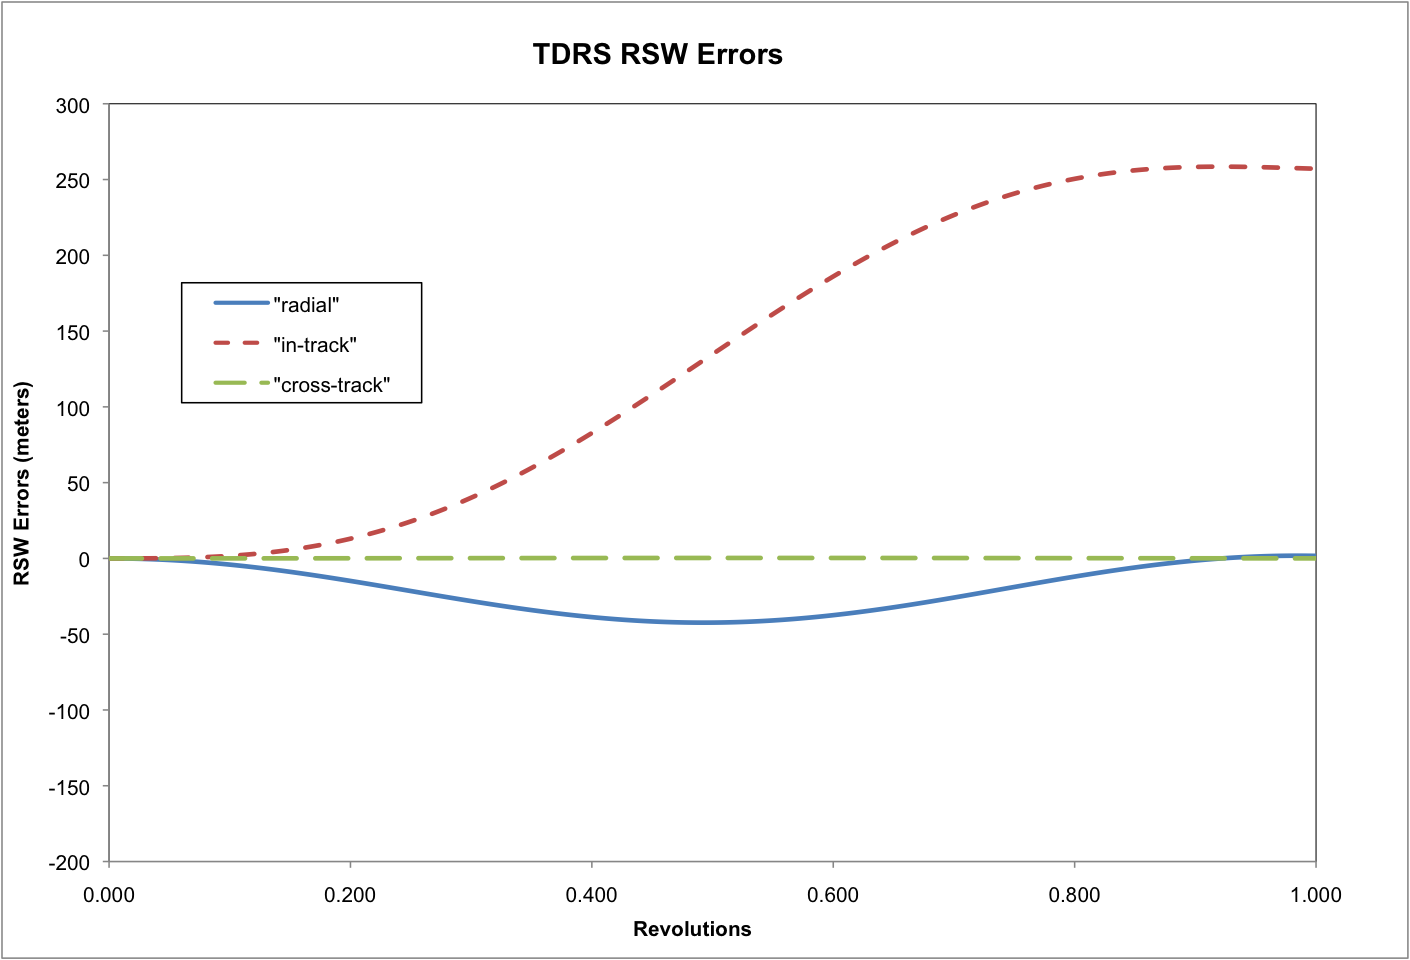
\includegraphics [width=7.0in]{figs/tdrs/tdrs_err.png}
\end{center}
\caption{TDRS RSW errors between measured and simulated orbit using GGM02C.}
\label{fig:5}
\end{figure}

\clearpage
\pagebreak
\end{description}

\subsection{Lunar Orbit:}
\test{Integrated Testing Clementine}\label{test:clem}
\begin{description}
\item[Introduction:] \ \newline
The Clementine spacecraft was built at the US Naval Research Laboratory in Washington,
DC, and carried sensors, attitude control systems, and software designed and built by the
Lawrence Livermore National Laboratory (LLNL). The US Air Force supplied advanced lightweight
composite structures and the launch vehicle, a Titan IIB refurbished ICBM. Several other
organizations were involved, especially NASA, with communications support, through the Jet
Propulsion Laboratory's (JPL) Deep Space network, and orbit determination and operations
support came from both the Goddard Space Flight Center and JPL. The spacecraft consists of
an octagonal prism about 2 meters high. A thruster for delta-V maneuvers is on one end
of the prism and a high-gain fixed dish antenna is on the other end. Clementine was launched
on January 25, 1994 from Vandenberg Air Force Base aboard a Titan IIB rocket. After two Earth
flybys, lunar insertion was achieved on February 19th. Lunar mapping took place over approximately
2 months in two systematic mapping passes over the Moon, semi major axis 5,116.0 km, eccentricity
0.36 and inclination of 90 degrees.
\item[Procedure:]\ \newline
An initial and final precision fit state vectors were obtained from JPL's SPICE data sets for
Clementine \cite{clem}.  The gravitational field is LP150 \cite{Knop}, and the field is
truncated to 60x60. Radiation pressure is modeled using a simple constant area. See the
appendix table \ref{tbl:clemic}.
\item[Results:]\ \newline
The radial error after 4.8 revolutions of Clementine is 60.6 meters, the in-track error
is 416.0 meters and the cross-track error is 5.3 meters see figure \ref{fig:6}. There are
several contributing factors to the in-track error: (1) The orbit fit of the measured data
has a large error in the in-track component of 30 meters, (2) The lunar gravitational
field is very complicated and gravitational models are still being refined \cite{Knop}
(increasing the degree and order of the model to 150x150 did not change to error results).
The spacecraft is modeled as a cannonball not as a complex spacecraft for radiation pressure
purposes which contributes some error. Figure \ref{fig:6} exhibits the fact that there is
shadowing by the Moon, most noticeable in the in-track component. Solar and earth third body
perturbations dominate the high eccentricity of Clementine orbit. This test partially satisfies
\ref{reqt:main_function}, \ref{reqt:rel_states}, and \ref{reqt:sim_interface}.

\begin{figure}
\begin{center}
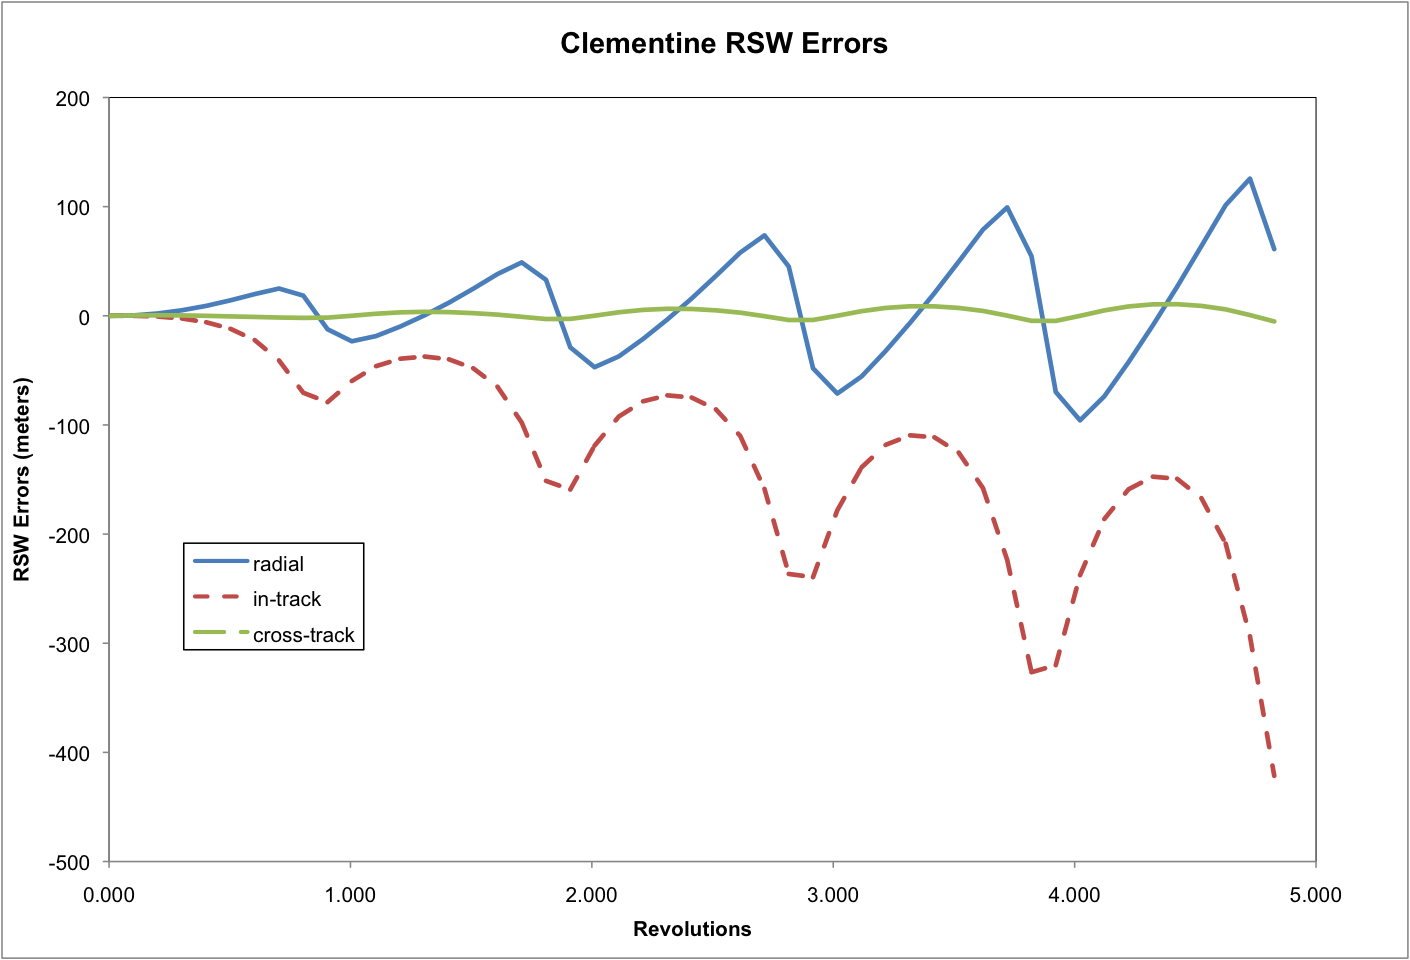
\includegraphics [width=7.0in]{figs/clem/clem_err.png}
\end{center}
\caption{RSW errors accumulated over 4.8 revolutions (5 hr period) .}
\label{fig:6}
\end{figure}

\end{description}
\clearpage
\newpage

\subsection{Earth Orbit:}
\test{Integrated Testing Grace}\label{test:grace}
\begin{description}
\item[Introduction:] \ \newline
The Gravity Recovery and Climate Experiment (GRACE) is a dedicated spaceborne mission
to map the Earth's gravity field with unprecedented accuracy. The GRACE mission was
launched in March 2002, for a lifetime of approximately 5 years. It consists of two satellites,
co-orbiting in nearly polar orbit, at approximately 300-500 km altitude, separated by 100-500 km
along track. Primary measurements are the range change between the two satellites, which represents
the gravity perturbation differences between the two locations. These range changes are measured
by a high accuracy microwave raging system. To detect the non-gravitational perturbations, which
also affect the range change, three axis accelerometers are used. The satellites are known as Grace A and Grace B.
\item[Procedure:]\ \newline
The benchmark precision orbit was obtained from Dr. John Ries \cite{JR} Center for Space Research
at the University of Texas. The data was for one day (October 2 2002) starting at midnight. The
state vector data was provided in 5 second intervals for both Grace A and Grace B. Earth gravity
was modeled up to 36x36 terms, atmosphere was modeled using the MET atmosphere , and the Moon and
Sun were third body perturbers. This simulation is a separate directory under Integrated\_Validation
as Sim\_grace and has it's own S\_define. See the appendix tables \ref{tbl:gracea}, \ref{tbl:graceb}
\item[Results:]\ \newline
The RSW errors for both Grace A and Grace B are shown in figures \ref{fig:7} and  \ref{fig:8}. The
two error histories are essentially the same as would be expected, since the two vehicles are in the
same orbit. The in-track error is nearly 11 km after one day and fairly negligible in radial and
cross-track. The benchmark measured data was in the year of the launch during a period of high solar
activity. The ballistic coefficient value used in the simulation was estimated based on the mass of the
vehicles, the projected area, and the coefficient of drag \cite{JR}. However it is known that there is
variation in the simple projected area drag model \cite{maz}. The ballistic coefficient was varied and
one can change the error; however, this is an objective of a future study. For now the user is presented
with this canonical value and the errors are the metrics which, for now, characterize the JEOD modeling.
This test partially satisfies \ref{reqt:main_function}, \ref{reqt:rel_states}, and \ref{reqt:sim_interface}.

\begin{figure}
\begin{center}
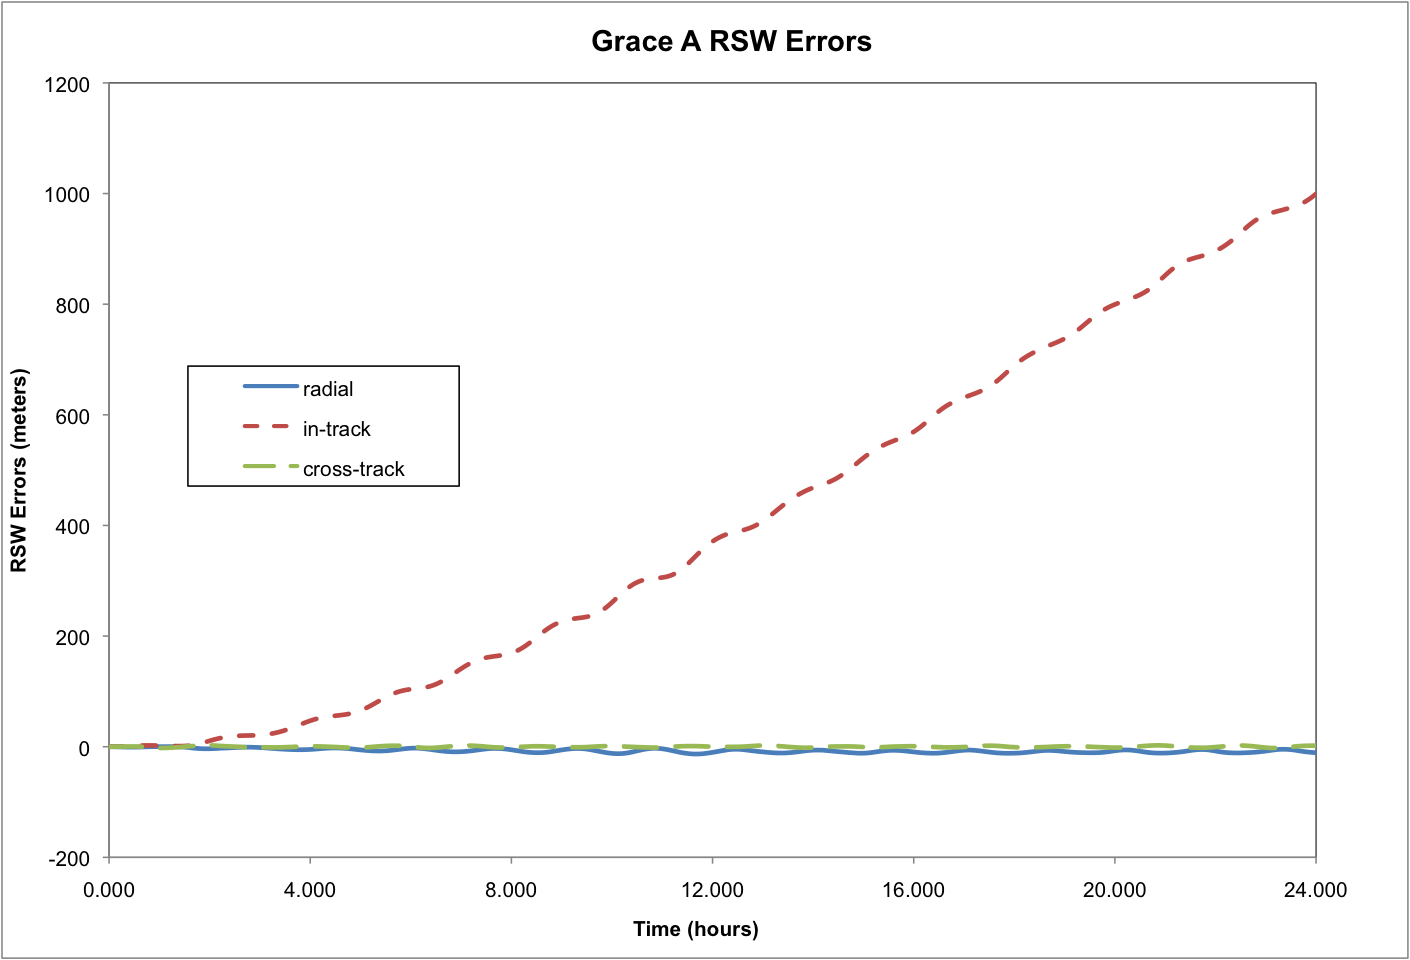
\includegraphics [width=7.0in]{figs/grace/gracea_err.png}
\end{center}
\caption{Grace A RSW errors accumulated over one day .}
\label{fig:7}
\end{figure}

\begin{figure}
\begin{center}
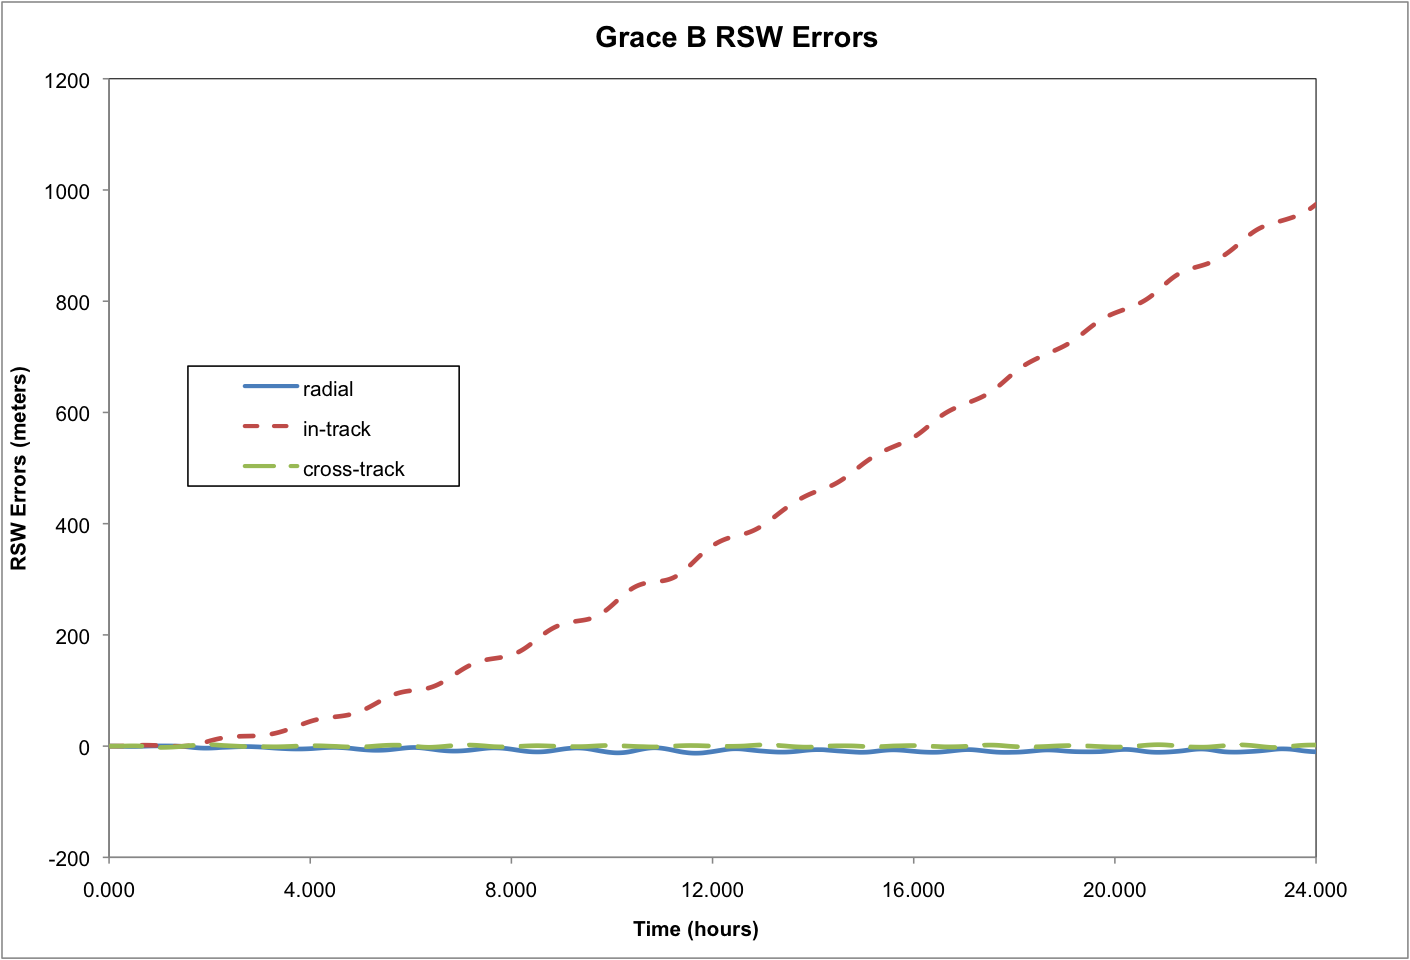
\includegraphics [width=7.0in]{figs/grace/graceb_err.png}
\end{center}
\caption{Grace B RSW errors accumulated over one day .}
\label{fig:8}
\end{figure}

\end{description}
\clearpage
\newpage

\test{Integrated Testing Rosetta}\label{test:rosetta}
\begin{description}
\item[Introduction:] \ \newline
Rosetta is a European Space Agency-led robotic spacecraft mission launched in 2004,
intended to study the comet 67P/Churyumov-Gerasimenko. Launched in March 2004 with
an Ariane-5/G1 it utilizes four planetary swingby maneuvers (gravity assists) in order
to get the correct Earth escape velocity to reach the comet in May 2014.  The second
swingby, around Mars, took place on 25 February 2007.
\item[Procedure:]\ \newline
Data were obtained from the JPL Horizons system for the Earth gravity assist maneuver.
The benchmark data starts about 5 min. before entry into the Earth's activity sphere and
end about 7 hours later. Rosetta passed at about 5000 km altitude. The modeled forces were
Earth gravity up to the J20 harmonic with Lunar and Solar perturbations and without atmosphere
or radiation effects. This test exists as a run in the directory Sim\_Earth\_Moon. See the
appendix table \ref{tbl:rosetta}
\item[Results:]\ \newline
As can be seen in Figure \ref{fig:9}, in this Earth flyby, the RSW error is small before
the swingby. The radial error remains relatively small but the in-track grows to more than
8 km while the off-track is on the order of 30 km. This simulation verifies that one may set
up and propagate a hyperbolic orbit about the Earth. As of this writing the source of the
RSW errors is not quite understood.  It may be a consequence of using the RK4 numerical
integrator; however, it may be some consequence of modeling. It is noted that the simulation
only missed the altitude of closest approach by less than a kilometer. The user is presented
with this test and its result as a measure of this simulation.  This test partially satisfies
\ref{reqt:main_function}, \ref{reqt:rel_states}, and \ref{reqt:sim_interface}.


\begin{figure}
\begin{center}
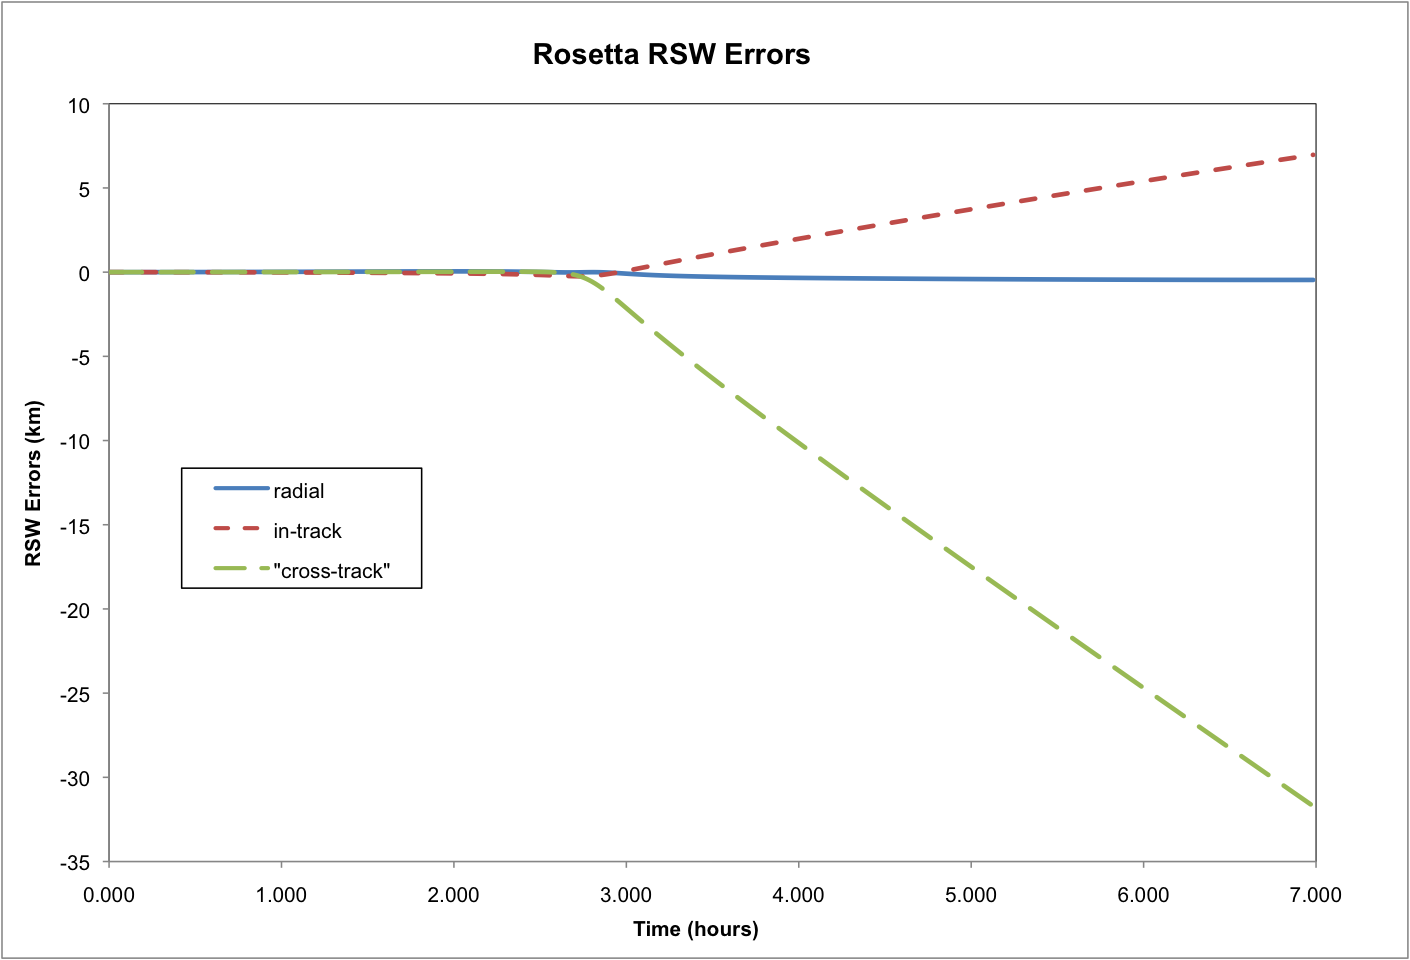
\includegraphics [width=7.0in]{figs/rosetta/rosettaerr.png}
\end{center}
\caption{RSW errors accumulated over 7 hours  .}
\label{fig:9}
\end{figure}

\end{description}
\clearpage
\newpage

\subsection{Mars Orbit: }
\test{Integrated Testing Phobos}\label{test:phobos}
\begin{description}
\item[Introduction:] \ \newline
Phobos is a natural satellite of Mars who's origin is  debated. However, Phobos's orbit has
been extensively studied and accurate models exist that describe its orbit. Phobos is orbiting
Mars in a nearly circular, and near equatorial orbit.  It has an inclination of 1.075 degrees
with respect to the equator and an eccentricity of 0.01515.  Its mean distance to Mars is only
9375 km or approximately 6000 km above the surface of Mars which has a mean radius of 3389.5 km.
At this close distance it is dynamically tied to the gravity field of Mars.
\item[Procedure:]\ \newline
Data was obtained from the JPL Horizons system for 24 of Phobos orbit with a data point every 10
minutes. The modeled forces were Mars non-spherical gravity with Solar perturbations. The simulation
did not include atmosphere, radiation forces, Phobos libration or gravitation effects of other
planets such as Jupiter.

See the appendix table \ref{tbl:phobos}
\item[Results:]\ \newline
As can be seen in Figure \ref{fig:10}, JEOD does fairly well in tracking the motion of Phobos.
The final error in the moon's in-track position of close to 200 meters is much smaller than Phobos
itself, which measures 13.4 X 11.2 X 9.2 km. This test partially satisfies \ref{reqt:main_function},
\ref{reqt:rel_states}, and \ref{reqt:sim_interface}.


\begin{figure}
\begin{center}
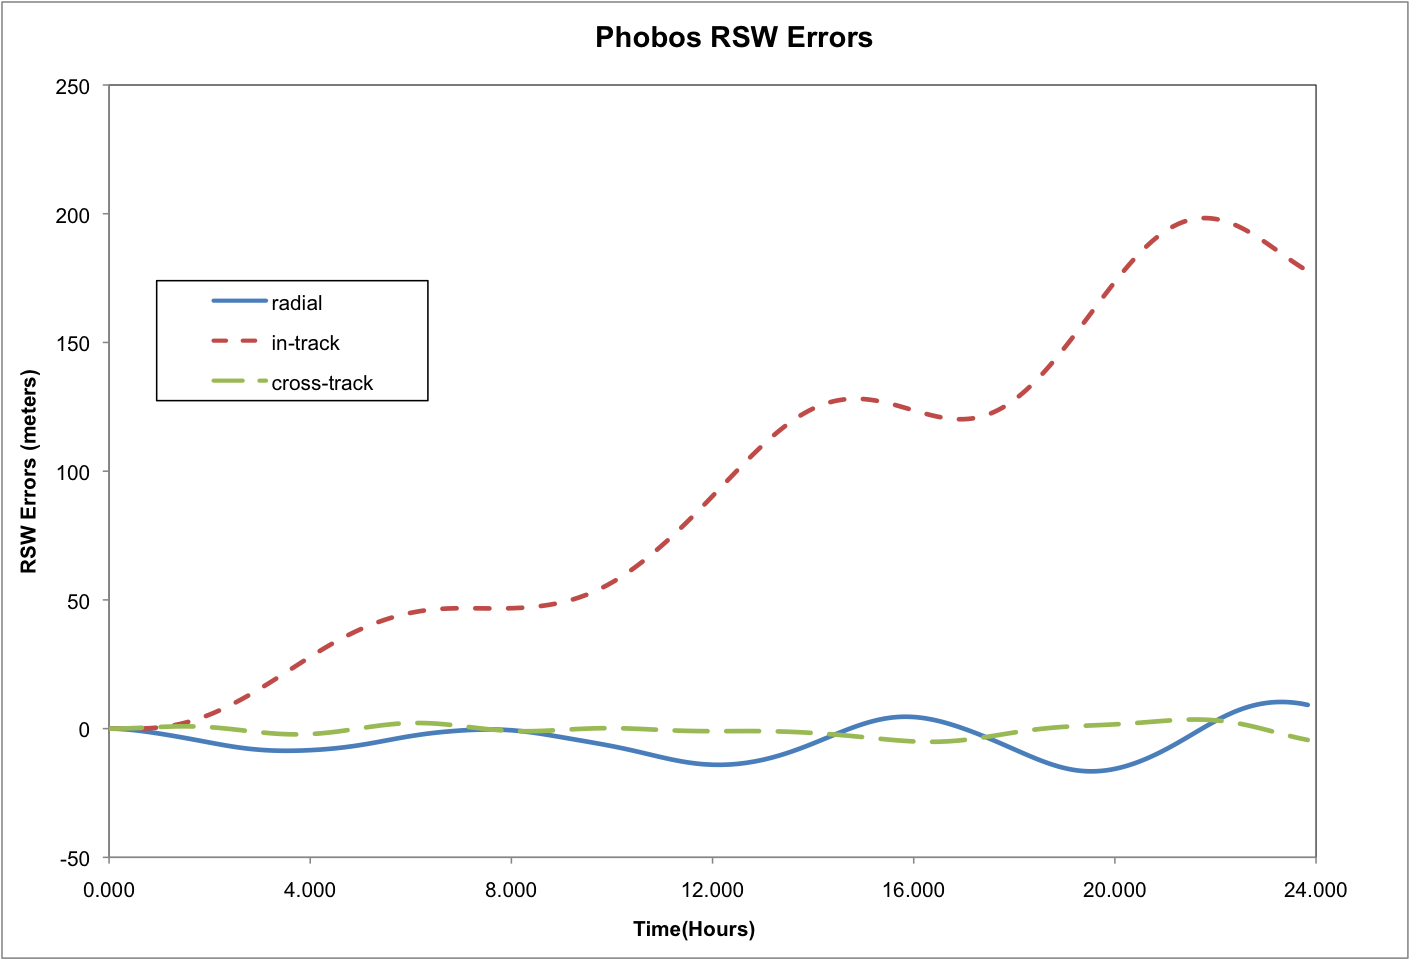
\includegraphics [width=7.0in]{figs/phobos/phobos_err.png}
\end{center}
\caption{RSW errors accumulated over 24 hours.}
\label{fig:10}
\end{figure}

\end{description}
\clearpage
\newpage

\test{Integrated Testing Dawn}\label{test:dawn}
\begin{description}
\item[Introduction:] \ \newline
Dawn is an ion-propelled spacecraft capable of visiting multiple targets in the main asteroid belt.
In the baseline mission, Dawn flies to and orbits the main belt asteroids 1 Ceres and 4 Vesta,
orbiting Vesta for a period of not less than seven months and Ceres for not less than five months.
The spacecraft flies by Mars in a gravity assist maneuver in 2009 en route to Vesta. The purpose of
the Mars gravity assist is to add energy to the spacecraft trajectory to ensure adequate mass and
power margins for the designated trajectory. The swingby event had no maneuver events.
\item[Procedure:]\ \newline
Data were obtained from the JPL Horizons system for the Mars gravity assist maneuver. The benchmark
data start about 1.5 hours before entry into the Mars closest approach and ends about 1.5 hours later.
Dawn passed at about a 550 km altitude. The modeled forces were Mars non-spherical gravity with Solar
perturbations and without atmosphere or radiation forces.

See the appendix table \ref{tbl:dawn}
\item[Results:]\ \newline
As can be seen in Figure \ref{fig:11}, in this Mars flyby the RSW error is small before the swingby.
The post encounter radial error is relativity small, the cross-track is about 3km but the in-track
grows to more than 6 km. This simulation verifies that one may set up and propagate a hyperbolic
orbit about Mars. As of this writing the source of the RSW errors is not quite understood, it may
be a consequence of using the RK4 numerical integrator, however it may be some consequence of modeling.
That the simulation only missed the altitude of closest approach by less than a kilometer. The user
is presented with this test and its result as a measure of this simulation.  This test partially
satisfies \ref{reqt:main_function}, \ref{reqt:rel_states}, and \ref{reqt:sim_interface}.


\begin{figure}
\begin{center}
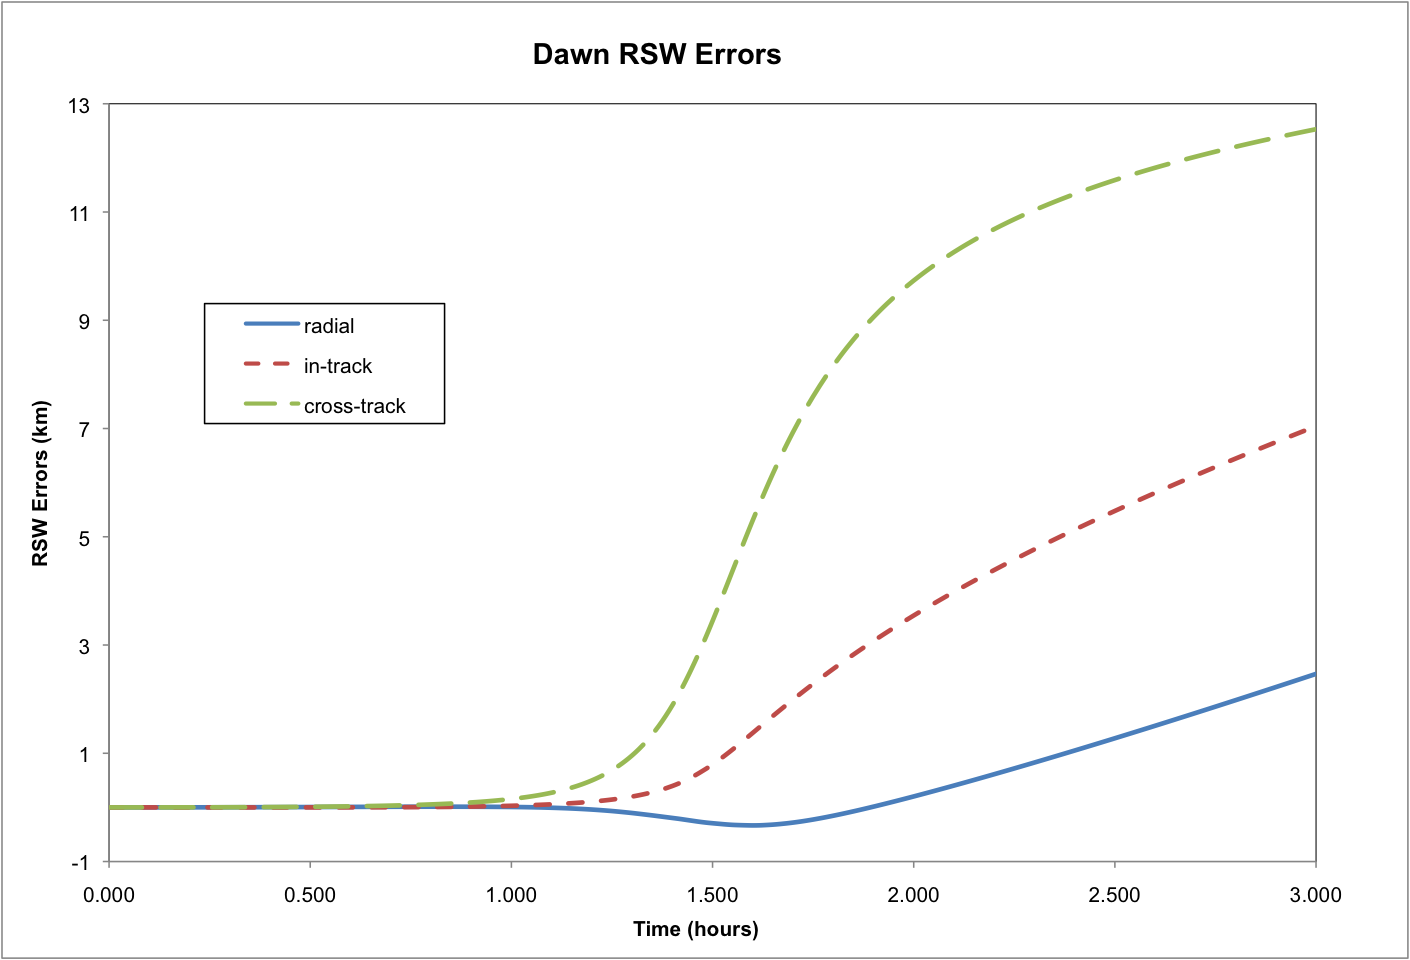
\includegraphics [width=7.0in]{figs/dawn/dawn_enc.png}
\end{center}
\caption{RSW errors accumulated over 3 hours.}
\label{fig:11}
\end{figure}

\end{description}
\clearpage
\newpage


\section{Requirements Traceability}\label{sec:traceability}

\begin{table}[ht]
\centering
\caption{Requirements Traceability}
\begin{tabular}{||l|l|l|} \hline
{\bf Requirement} & {\bf Inspection or test} \\ \hline \hline
\ref{reqt:documentation} - Documentation &
  Insp. \ref{inspect:documentation} - Documentation \\ \hline
\ref{reqt:jeod_code} - JEOD code &
  Insp. \ref{inspect:code} - JEOD Coding Standards \\ \hline
\ref{reqt:main_function} - Main Function &
  Test \ref{test:champ} and all other JEOD Integrated Validation Simulations \\ \hline
\ref{reqt:rel_states} - Relative States &
Test \ref{test:champ} and all other JEOD Integrated Validation Simulations \\ \hline
\ref{reqt:sim_interface} - Simulation Interface &
Test \ref{test:champ} and all other JEOD Integrated Validation Simulations \\ \hline
\hline
\end{tabular}
\end{table}


\section{Code Coverage}\label{sec:code_coverage}
JEOD contains code coverage report for the entire software in HTML format,
which can be found by opening ``index.html" located at top level
``artifact/coverage/coverage\_results" directory. Code coverage report is
generated using LCOV.
